
%***************************************************************************
%
% CreditCruncher - A portfolio credit risk valorator
% Copyright (C) 2004 Gerard Torrent
%
% This program is free software; you can redistribute it and/or
% modify it under the terms of the GNU General Public License
% as published by the Free Software Foundation; either version 2
% of the License.
%
% This program is distributed in the hope that it will be useful,
% but WITHOUT ANY WARRANTY; without even the implied warranty of
% MERCHANTABILITY or FITNESS FOR A PARTICULAR PURPOSE.  See the
% GNU General Public License for more details.
%
% You should have received a copy of the GNU General Public License
% along with this program; if not, write to the Free Software
% Foundation, Inc., 59 Temple Place - Suite 330, Boston, MA 02111-1307, USA.
%
%
% implementation.tex - TeX documentation file
% --------------------------------------------------------------------------
%
% 2005/01/22 - Gerard Torrent [gerard@fobos.generacio.com]
%   . initial release
%
%***************************************************************************

\chapter{Implementaci\'on de la soluci\'on}
\label{sec:implementation}

\section{Validaciones}

TODO: describir las validaciones realizadas


\begin{figure}[!hb]
\begin{center}
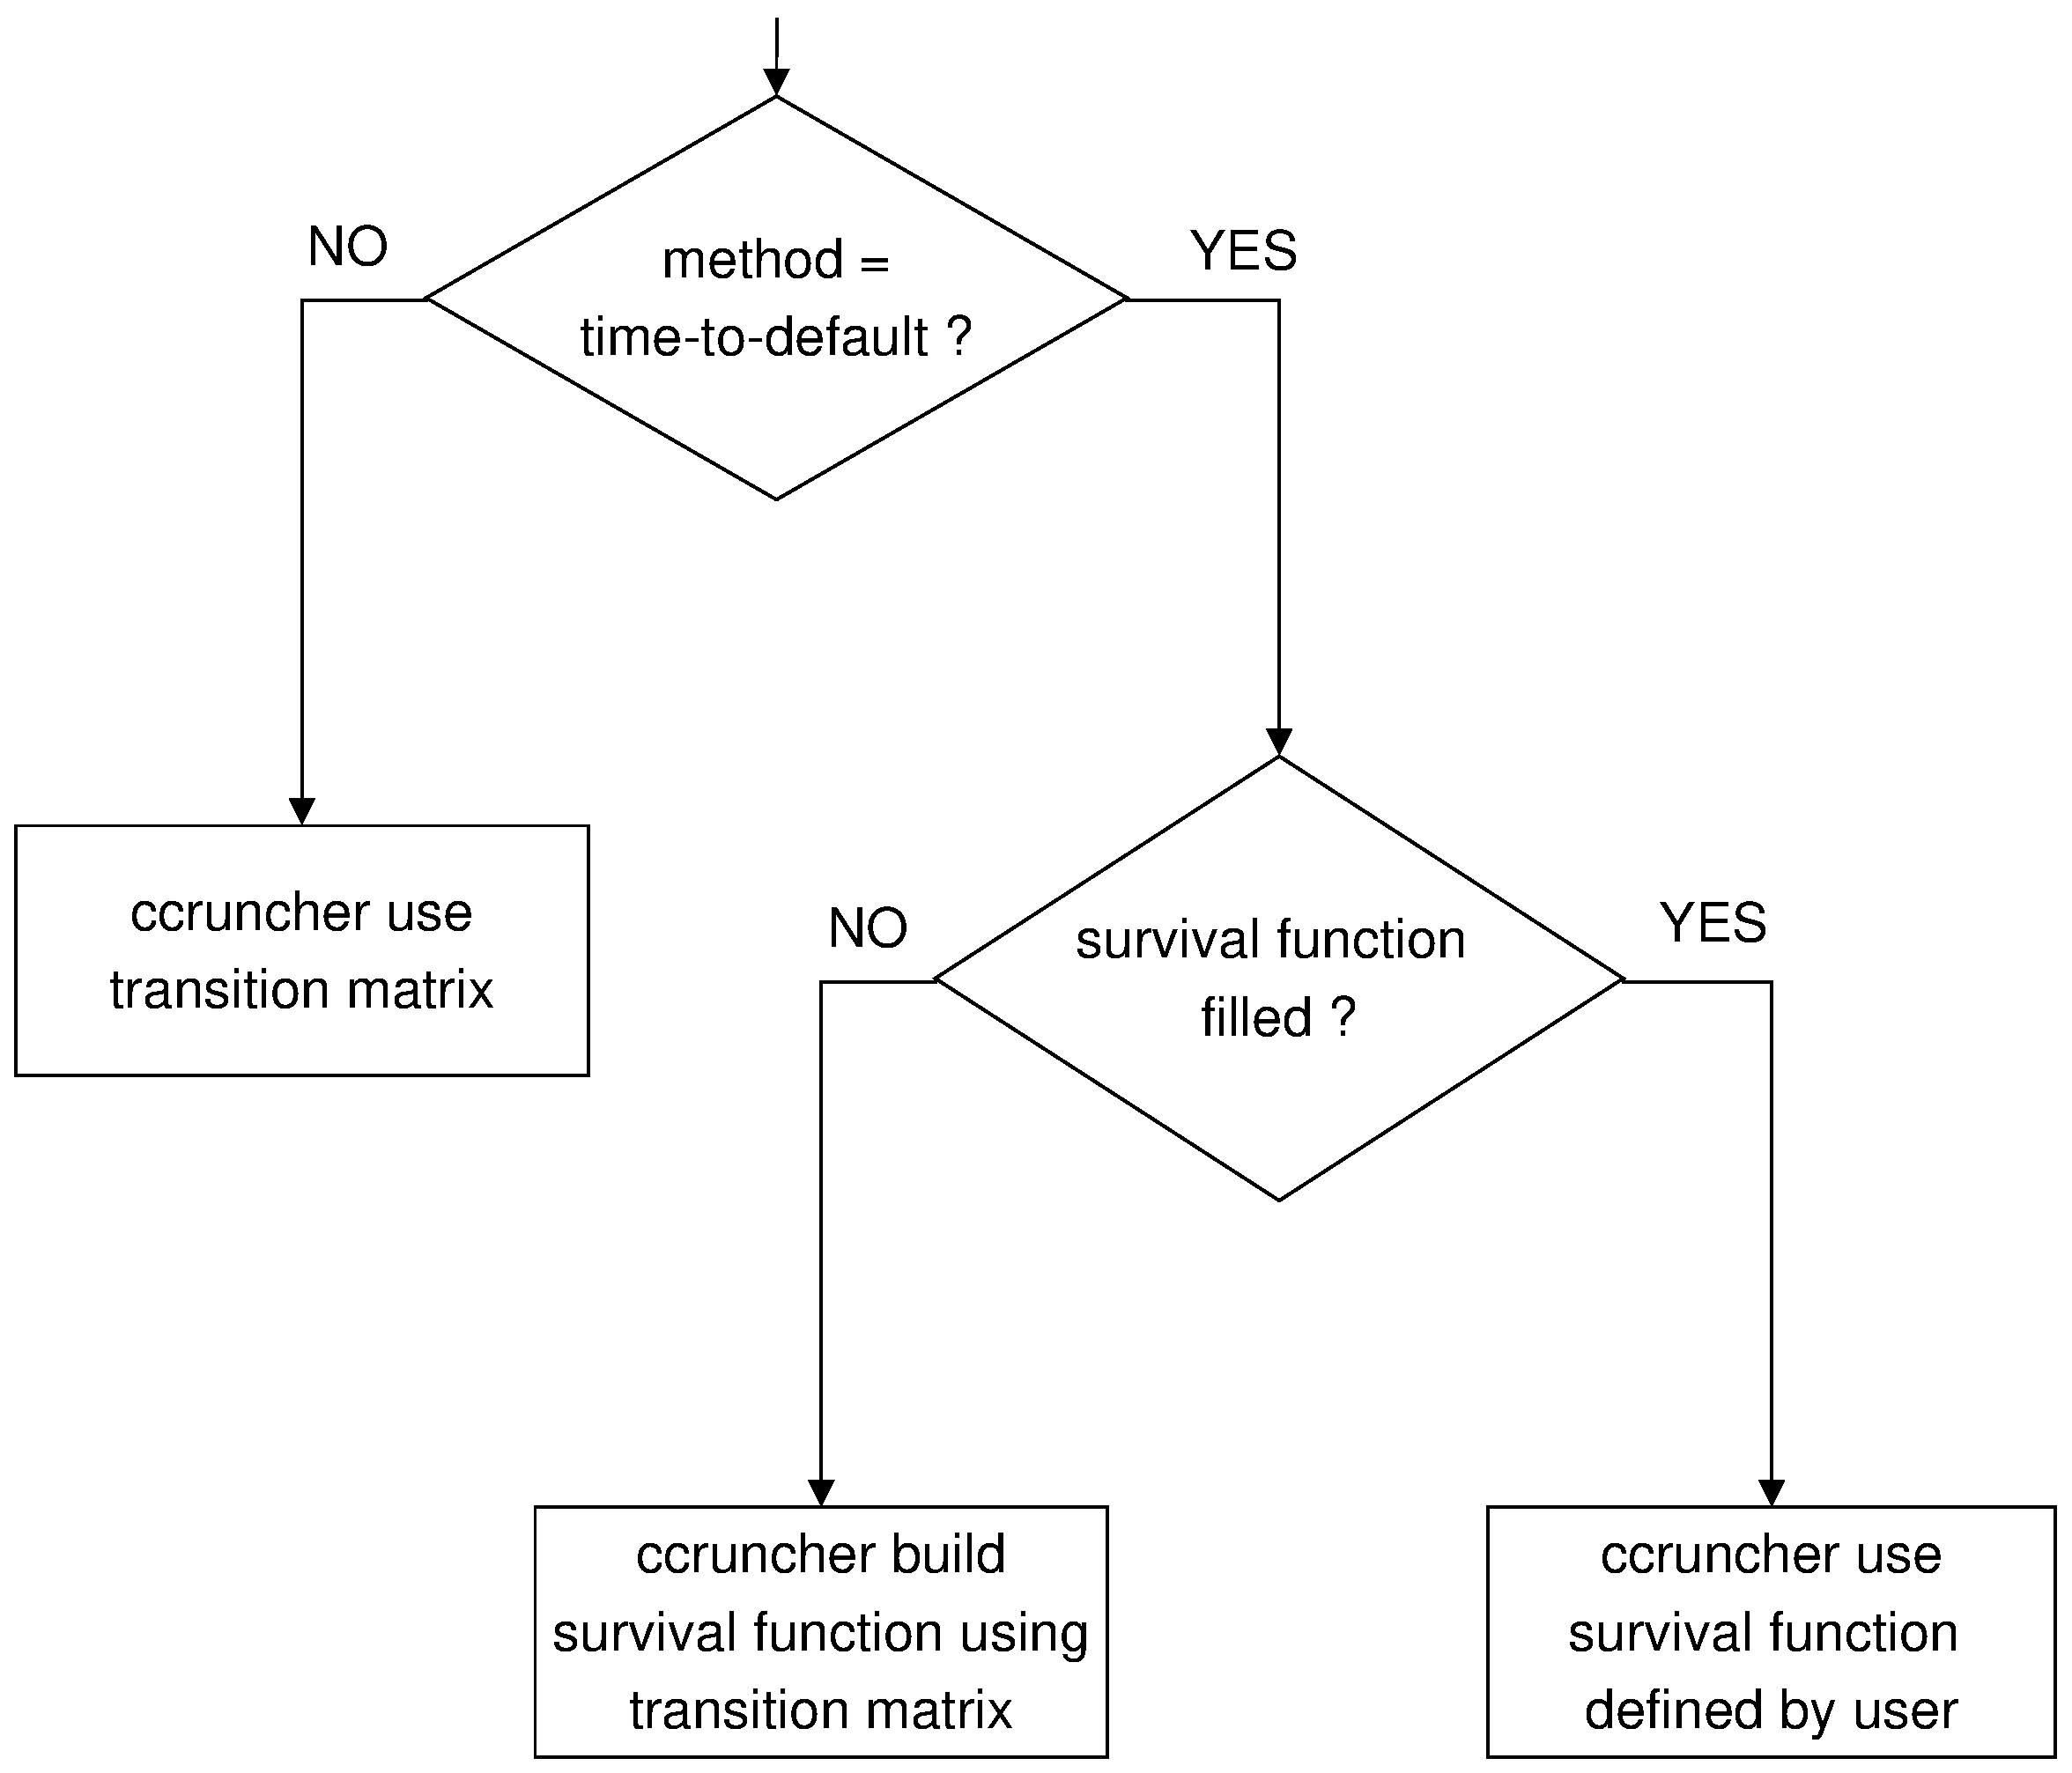
\includegraphics[width=10cm,angle=0]{./images/decisiontree1.eps}
\caption{Decisi\'on en funci\'on del m\'etodo}
\label{functionsIJ}
\end{center}
\end{figure}


\section{Proceso de agregaci\'on}

TODO: descripcion de los agregadores y metodo usado para evitar recalculo 
de los activos en cada simulacion + Agregaci\'on de productos


\section{Dimensiones del problema}

TODO: Estimaciones de uso de memoria, estimaci\'on del numero de operaciones,
estimacion del tiempo de computo


\section{Convergencia de la soluci\'on}

TODO: N\'umero de iteraciones necesarias, aceleraci\'on de la convergencia
usando metodolog\'ia antithetic

